

\section{Математичне та алгоритмічне забезпечення аналітичної системи}

\subsection{Структура та граф взаємодії компонентів програмно-алгоритмічного конвеєра}

Проектування високонавантажених систем комп'ютерного зору вимагає
чіткої декомпозиції алгоритмічних кроків для виключення затримок передачі
даних. Розроблена система побудована за модульним принципом, де кожен
етап оперує строго типізованими математичними тензорами.

\begin{figure}[!htbp]
    \centering
    \label{fig:algorythm_structure}
    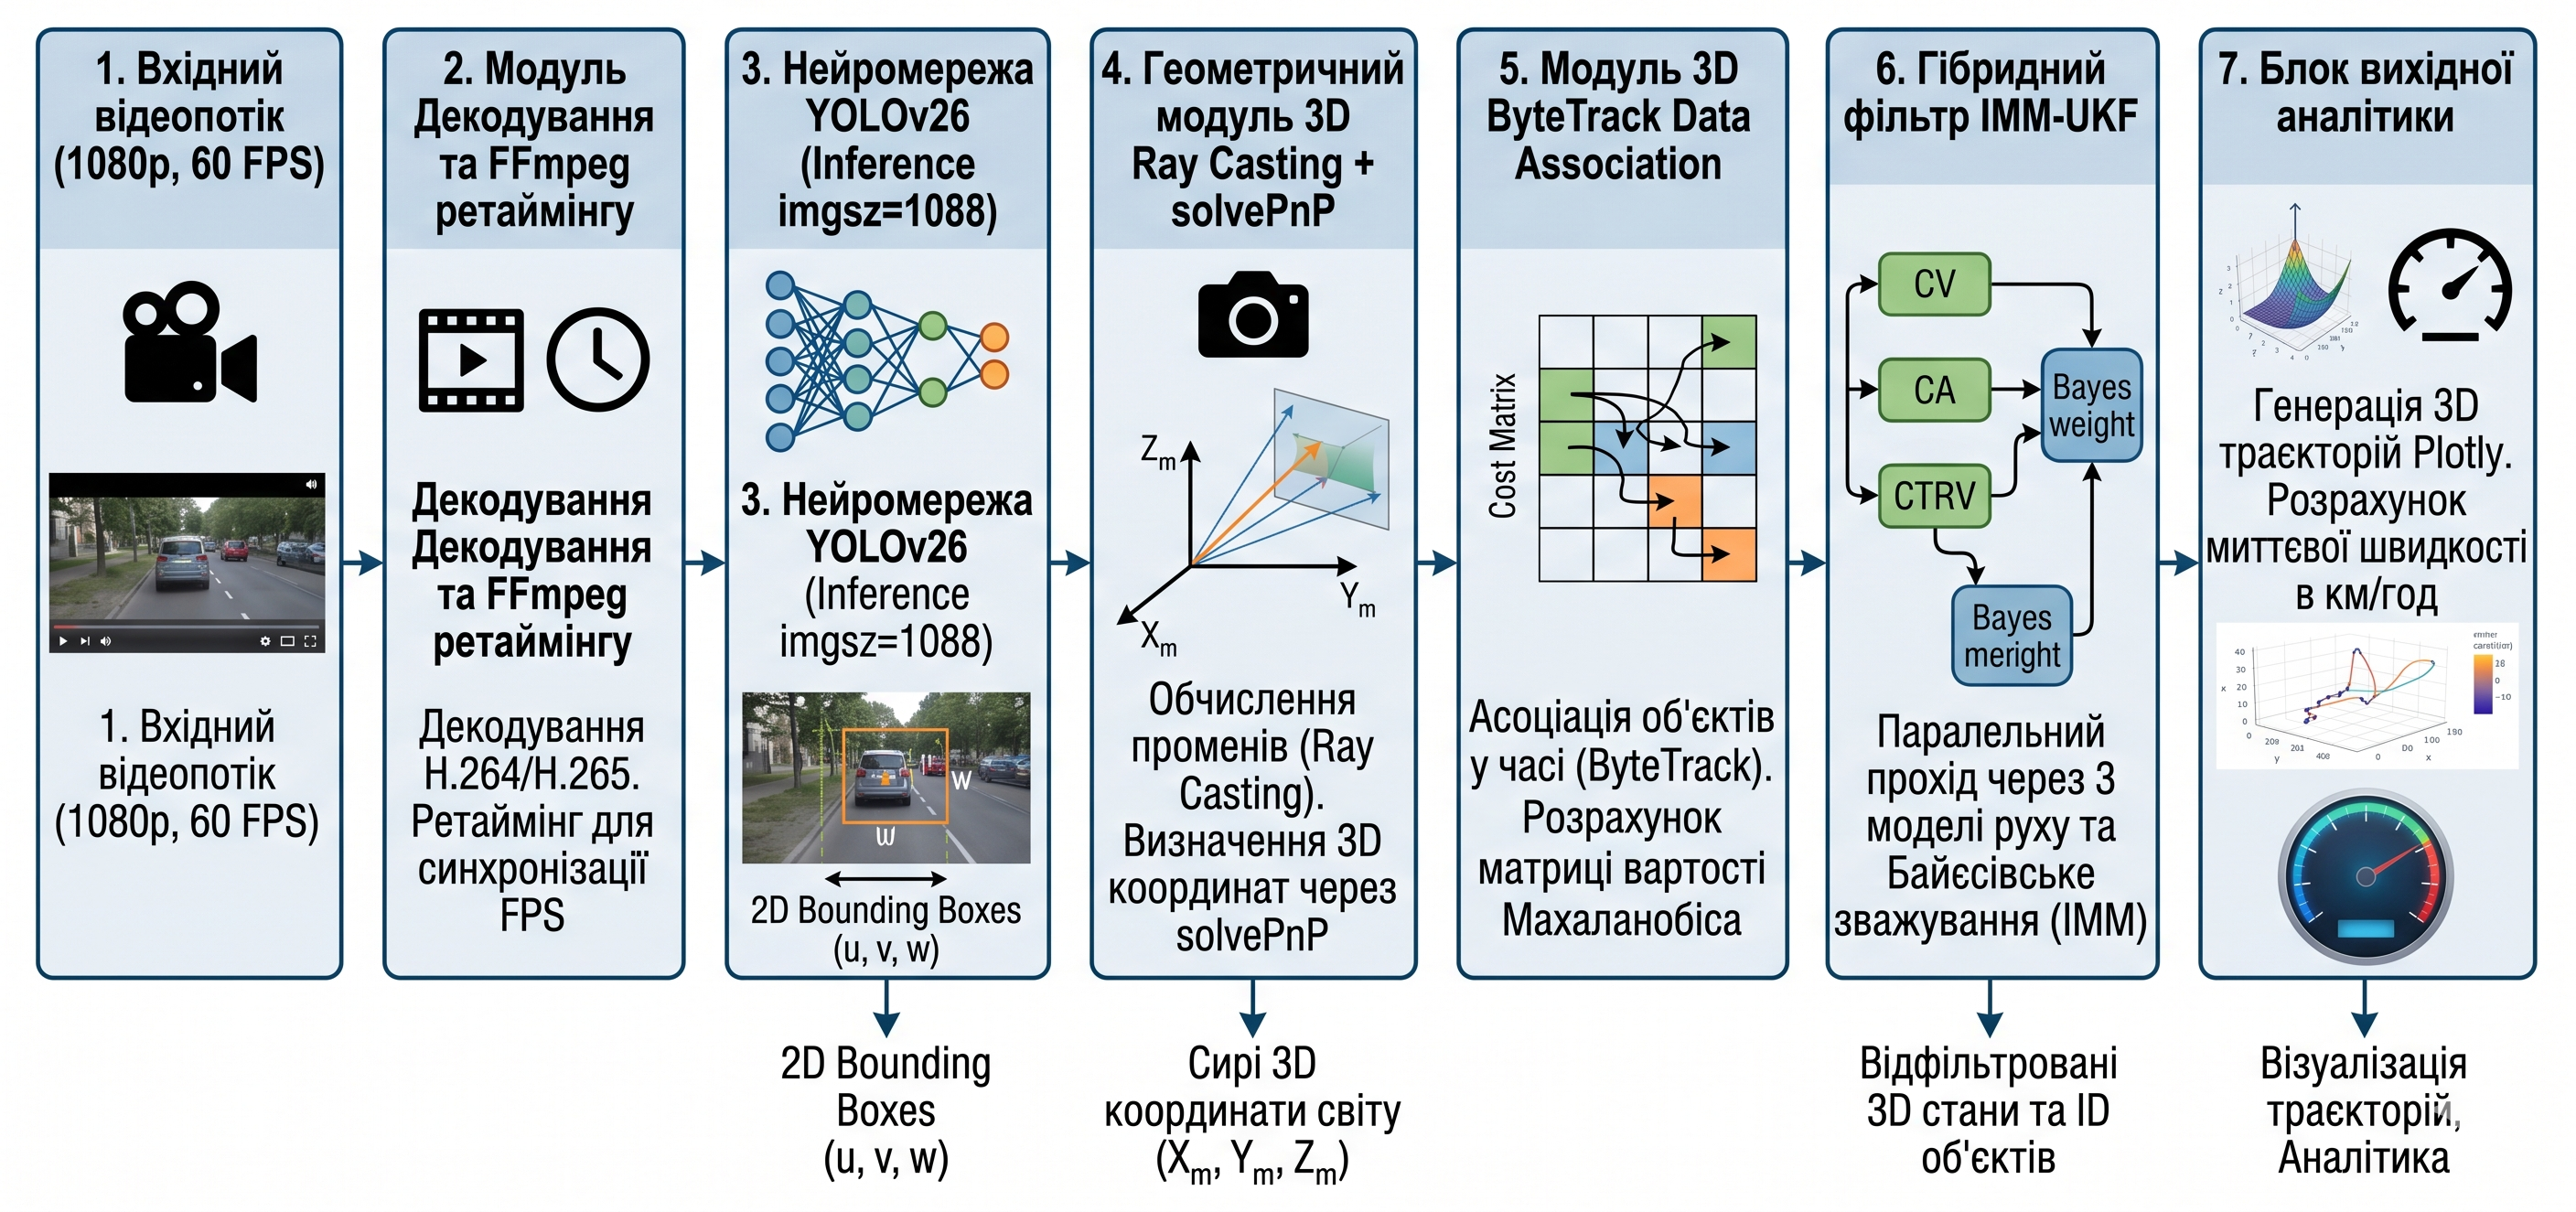
\includegraphics[width=\textwidth]{sections/pictures_schemes/chapter_2/2_1_algorythmic_conveyer_structure}
    \caption{Загальна архітектура конвеєра обробки відео для 3D-відстеження об'єктів}

\end{figure}


\subsection{Математична модель геометричного зворотного проектування
та вирівнювання базису осей}

Для просторового калібрування камери використовується система
рівнянь перспективної проєкції. Матриця внутрішніх параметрів камери K
задається як:
\[K = \begin{bmatrix} f_x & 0 & c_x \ 0 & f_y & c_y \ 0 & 0 & 1 \end{bmatrix},\]
де $f_x$, $f_y$ — фокальні відстані в пікселях, а $c_x$, $c_y$ — координати
головної точки (оптичного центру) на матриці. Алгоритм `cv2.solvePnP`
мінімізує похибку зворотного проектування(Reprojection Error) для множини реперних точок розмітки поля, повертаючи
матрицю обертання $R \in S0(3)$ та
вектор зсуву t.
Для реалізації методу Ray Casting піксельні координати детекції центру
м'яча $[u, v, 1]^T$ трансформуються в нормалізований вектор напрямку в
системі координат камери: $d_{cam} = K^{-1} [u, v, 1]^T$. Переведення цього
вектора у глобальну систему координат залу здійснюється шляхом множення
на обернену (транспоновану) матрицю обертання $R^T$:
\[d_{world} = R^T \cdot d_{cam} = R^T \cdot \begin{bmatrix} \frac{u - c_x}{f_x} \ \frac{v -
c_y}{f_y} \ 1 \end{bmatrix}.\]
Фізична позиція оптичного центру камери у просторі світу визначається
як $C = -R^T \cdot t$. Тоді будь-яка точка на промені описується функцією
глибини $Z_c$:
\[P(Z_c) = C + Z_c \cdot d_{world}.\]
Для однозначного визначення масштабу $Z_c$ використовується відома
фізична константа — діаметр волейбольного м'яча $D_{real} = 0.21$ м. Глибина
обчислюється через поточну піксельну ширину рамки детекції w: $Z_c = (f_x
\cdot D_{real}) / w.$
Рішення проблеми конфлікту осей: В оптичній системі координат
OpenCV вісь $Y_{cam}$ спрямована вниз від оптичного центру до підлоги,
а вісь $Z_{cam}$ — уперед вздовж оптичної осі. Натомість опорна базисна
система волейбольного корту, заданого реперними точками,
має наступну орієнтацію: вісь $X$ — поперек майданчика
(вздовж лицевої лінії), вісь $Z$ — вздовж довгої сторони
(вздовж бічної лінії), а вісь $Y$ — суто вертикальна, спрямована вгору
від поверхні підлоги проти вектора прискорення вільного падіння. Усі
реперні точки розмітки лежать у площині $Y = 0$. Сирий вектор $P_{raw} =
[X, Y, Z]^T$, отриманий зворотним проектуванням, має негативний знак
координати $Y$ для точок, розташованих над підлогою (через те, що камера
розміщена вище та дивиться вниз). Для приведення базису до фізично
коректного вигляду застосовується спрощений лінійний оператор
дзеркальної інверсії осі висоти $M_{align}$:
\[P_{court} = M_{align} \cdot P_{raw} = \begin{bmatrix} 1 & 0 & 0 \\ 0 & -1 & 0 \\ 0 & 0 & 1
\end{bmatrix} \begin{bmatrix} X \\ Y \\ Z \end{bmatrix} = \begin{bmatrix} X \\ -Y \\ Z
\end{bmatrix}.\]
Така трансформація дозволяє узгодити метричні дані з класичним
вектором прискорення вільного падіння $\vec{g} = [0,\, -9.81,\, 0]^T$ і у
подальшому використовувати вісь $Y$ як єдиний носій інформації про
висоту польоту м'яча, а пара $(X, Z)$ описує його горизонтальну
проекцію на підлогу майданчика.

\textbf{Математична формалізація похибки зворотного проектування.} Алгоритм
\gls{PnP} мінімізує сукупну евклідову відстань між істинною піксельною
координатою реперної точки $(u_i, v_i)$ та її проекцією за поточними
оцінками матриці обертання $R$ і вектора зсуву $t$:
\[\mathcal{L}_{reproj}(R, t) = \sum_{i=1}^{N} \left\| \begin{pmatrix} u_i \\ v_i \end{pmatrix} - \pi\left( K (R P_i + t) \right) \right\|^2,\]
де $P_i \in \mathbb{R}^3$ --- відома просторова координата $i$-ї реперної точки розмітки
поля, а оператор $\pi$ переводить однорідну тривимірну координату на площину сенсора за
правилом $\pi([x, y, z]^T) = [x/z, y/z]^T$. Внаслідок нелінійності функції $\pi$ та
матричної експоненти Родрігеса $R = \exp([\omega]_\times)$ задача мінімізації
$\mathcal{L}_{reproj}$ не має замкнутого аналітичного розв'язку. Метод Левенберга-Марквардта,
закладений у реалізацію \texttt{cv2.solvePnP}, ітераційно лінеаризує цільову функцію
навколо поточної оцінки параметрів та виконує крок градієнтного спуску у напрямку
зменшення квадратичної похибки. Збіжність зазвичай досягається за 8--15 ітерацій з
кінцевою середньоквадратичною похибкою репроекції $\sqrt{\mathcal{L}_{reproj}/N} < 1.5$
пікселя для типового набору з 4 реперних точок розмітки.

\textbf{Обґрунтування параметрів матриці внутрішніх параметрів $K$.} Для типової
аматорської камери з матрицею Sony IMX355 та фокальною відстанню об'єктива $f = 16$ мм
при пікселізації сенсора $p_s = 1.12 \cdot 10^{-3}$ мм/піксель фокальна відстань у
пікселях обчислюється як $f_x = f_y = f / p_s = 16 / (1.12 \cdot 10^{-3}) \approx 1300$
пікселів. Координати оптичного центру $c_x = W/2 = 960$ пікселів, $c_y = H/2 = 540$
пікселів обираються за припущенням, що оптична вісь проходить через геометричний центр
прямокутника сенсора. Зазначене припущення вносить додаткову систематичну похибку
проектування в межах $\pm 5$ пікселів через виробничу неточність позиціонування
світлочутливої матриці. Для більш точного калібрування може застосовуватися окрема
процедура з використанням еталонної шахової дошки (Zhang's method), проте у
розроблюваній системі такий рівень деталізації виявився надлишковим, оскільки
згладжуючий ефект сигма-точкового фільтра успішно поглинає піксельні похибки до 7--8
пікселів за стандартним відхиленням.

\textbf{Стохастична природа оцінки глибини.} Формула обчислення глибини
$Z_c = (f_x D_{real}) / w$ містить у знаменнику піксельну ширину рамки $w$, що сама
по собі є нелінійною функцією від положення центру об'єкта та від поточної впевненості
нейромережі. Шум $\delta w$ у визначенні ширини рамки трансформується у шум координати
глибини за законом $\delta Z_c \approx -(f_x D_{real} / w^2) \cdot \delta w$. При
типових значеннях $w \in [12, 80]$ пікселів цей коефіцієнт може досягати 1.9 м/піксель,
що пояснює необхідність окремого підвищення дисперсії шуму вимірювання $\sigma_z^2$ у
матриці $R$ порівняно з горизонтальними осями. Кількісно: $1$ піксель шуму ширини рамки
на відстані $15$ м $\Rightarrow$ помилка глибини $0.4-0.7$ м, що утричі перевищує
типовий діаметр об'єкта і тому обов'язково повинно бути відображено в априорних
параметрах фільтра.

\subsection{Математичний апарат \gls{UKF} та нелінійної аеродинаміки}

Вектор стану динамічної системи м'яча визначається у 6-вимірному просторі станів, що виключає необхідність
явного накопичення похибок прискорень як незалежних випадкових процесів:
\[x = [x, v_{x}, y, v_{y}, z, v_{z}]^{T}.\]

Рівняння переходу стану задаються системою першого порядку нелінійних диференціальних рівнянь, де прискорення
обчислюється функціонально через поточні компоненти швидкості, враховуючи силу тяжіння (що діє вздовж вертикальної осі
$Y$) та нелінійний квадратичний опір повітря (Drag Force):
\[\frac{d}{dt} \begin{bmatrix} x \\ v_x \\ y \\ v_y \\ z \\ v_z \end{bmatrix} = \begin{bmatrix} v_x \\
    -\frac{1}{2m}C_{d}\rho A ||v|| v_x \\ v_y \\ -\frac{1}{2m}C_{d}\rho A ||v|| v_y - g \\ v_z \\
    -\frac{1}{2m}C_{d}\rho A ||v|| v_z \end{bmatrix}\]
де $m=0.27$~кг --- маса волейбольного м'яча, $\rho=1.204$~кг/м$^{3}$ --- щільність повітря за стандартних умов,
$A=\pi(0.105)^{2}\approx0.0346$~м$^{2}$ --- площа міделевого перерізу об'єкта, $C_{d}\approx0.42$ --- коефіцієнт
лобового опору сфери у турбулентному потоці, а $g = 9.81$~м/с$^2$ --- прискорення вільного падіння. Зведений коефіцієнт
аеродинамічного опору $k = \frac{1}{2m}C_{d}\rho A \approx 0.0314$ с$^{-1}\cdot$м$^{-1}$ виноситься як стала перед
квадратичним членом $||v||$ і використовується у програмній реалізації моделі.

Для реалізації прогнозу в \gls{UKF} застосовується масштабоване сигма-точкове перетворення Ван дер Мерве. Для фактичної
розмірності стану системи $n=6$ генерується детермінований набір з $2n+1=13$ сигма-точок $\chi_{i}$ за формулами:
\begin{gather*}
    \chi_0 = \hat{x}, \\
    \quad \chi_i = \hat{x} + \left(\sqrt{(n + \lambda) P} \right)_i, \\
    \quad \chi_{i+n} = \hat{x} - \left(\sqrt{(n + \lambda) P} \right)_i,
\end{gather*}
де P — матриця коваріації помилки стану, а параметр масштабування
$\lambda = \alpha^2(n + \kappa) - n.$ Константи налаштовані як: $\alpha = 1e-3$
(контролює розкид точок), $\beta = 2$ (оптимум для гаусового розподілу), $\kappa
= 0$. Ваги для відновлення середнього значення $W_i^m$ та коваріації $W_i^c$
розраховуються як:
\begin{gather*}
    W_0^m = \frac{\lambda}{n + \lambda}, \\
    \quad W_0^c = \frac{\lambda}{n + \lambda} + (1 - \alpha^2 + \beta), \\
    \quad W_i^m = W_i^c = \frac{1}{2(n + \lambda)}.
\end{gather*}

Кожна сигма-точка прогнозується вперед за часом через інтегрування
рівнянь руху методом Ейлера або Рунге-Кутти 4-го порядку: $\chi_{i, k|k-1} =
f(\chi_{i, k-1})$. Побудова апріорного стану та коваріації виконується за
формулами:
\begin{gather*}
    \hat{x}_{k|k-1} = \sum_{i=0}^{2n} W_i^m \chi_{i, k|k-1}, \\
    \quad P_{k|k-1} = \sum_{i=0}^{2n} W_i^c \left[\chi_{i, k|k-1} - \hat{x}_{k|k-1} \right]\left[\chi_{i, k|k-1} - \hat{x}_{k|k-1}
    \right]^T + Q_k.
\end{gather*}

\textbf{Етап оновлення стану за вимірюванням.} На наступному
кроці $k$ після надходження нового вимірювання $z_k$ кожна
з 13 прогнозних сигма-точок $\chi_{i, k|k-1}$ пропускається
через функцію вимірювання $h(x) = [x_0, x_2, x_4]^T$, що
виокремлює саме просторові координати об'єкта без врахування
компонент швидкості. Результуючий набір трансформованих
сигма-точок $\mathcal{Z}_i = h(\chi_{i, k|k-1})$ використовується для
обчислення прогнозу вимірювання, інноваційної матриці
коваріації, перехресної коваріації стан-вимірювання та
підсилення Калмана:
\begin{gather*}
    \hat{z}_{k|k-1} = \sum_{i=0}^{2n} W_i^m \mathcal{Z}_i, \\
    S_k = \sum_{i=0}^{2n} W_i^c (\mathcal{Z}_i - \hat{z}_{k|k-1})(\mathcal{Z}_i - \hat{z}_{k|k-1})^T + R_k, \\
    P^{xz}_k = \sum_{i=0}^{2n} W_i^c (\chi_{i, k|k-1} - \hat{x}_{k|k-1})(\mathcal{Z}_i - \hat{z}_{k|k-1})^T, \\
    K_k = P^{xz}_k S_k^{-1}.
\end{gather*}
Постеріорна оцінка стану та її коваріація обчислюються
традиційним для фільтрів калманового сімейства способом:
\begin{gather*}
    \hat{x}_{k|k} = \hat{x}_{k|k-1} + K_k (z_k - \hat{z}_{k|k-1}), \\
    P_{k|k} = P_{k|k-1} - K_k S_k K_k^T.
\end{gather*}
Виражений вище алгоритм є замкненим і обчислюється за лінійний
від кількості сигма-точок час, що принципово виграє у часточкових
методів Монте-Карло, де щонайменше потрібно $N > 10^3$ часточок
для аналогічної точності оцінки коваріації.

\begin{figure}[!htbp]
    \centering
    \label{fig:unscented_transform}
    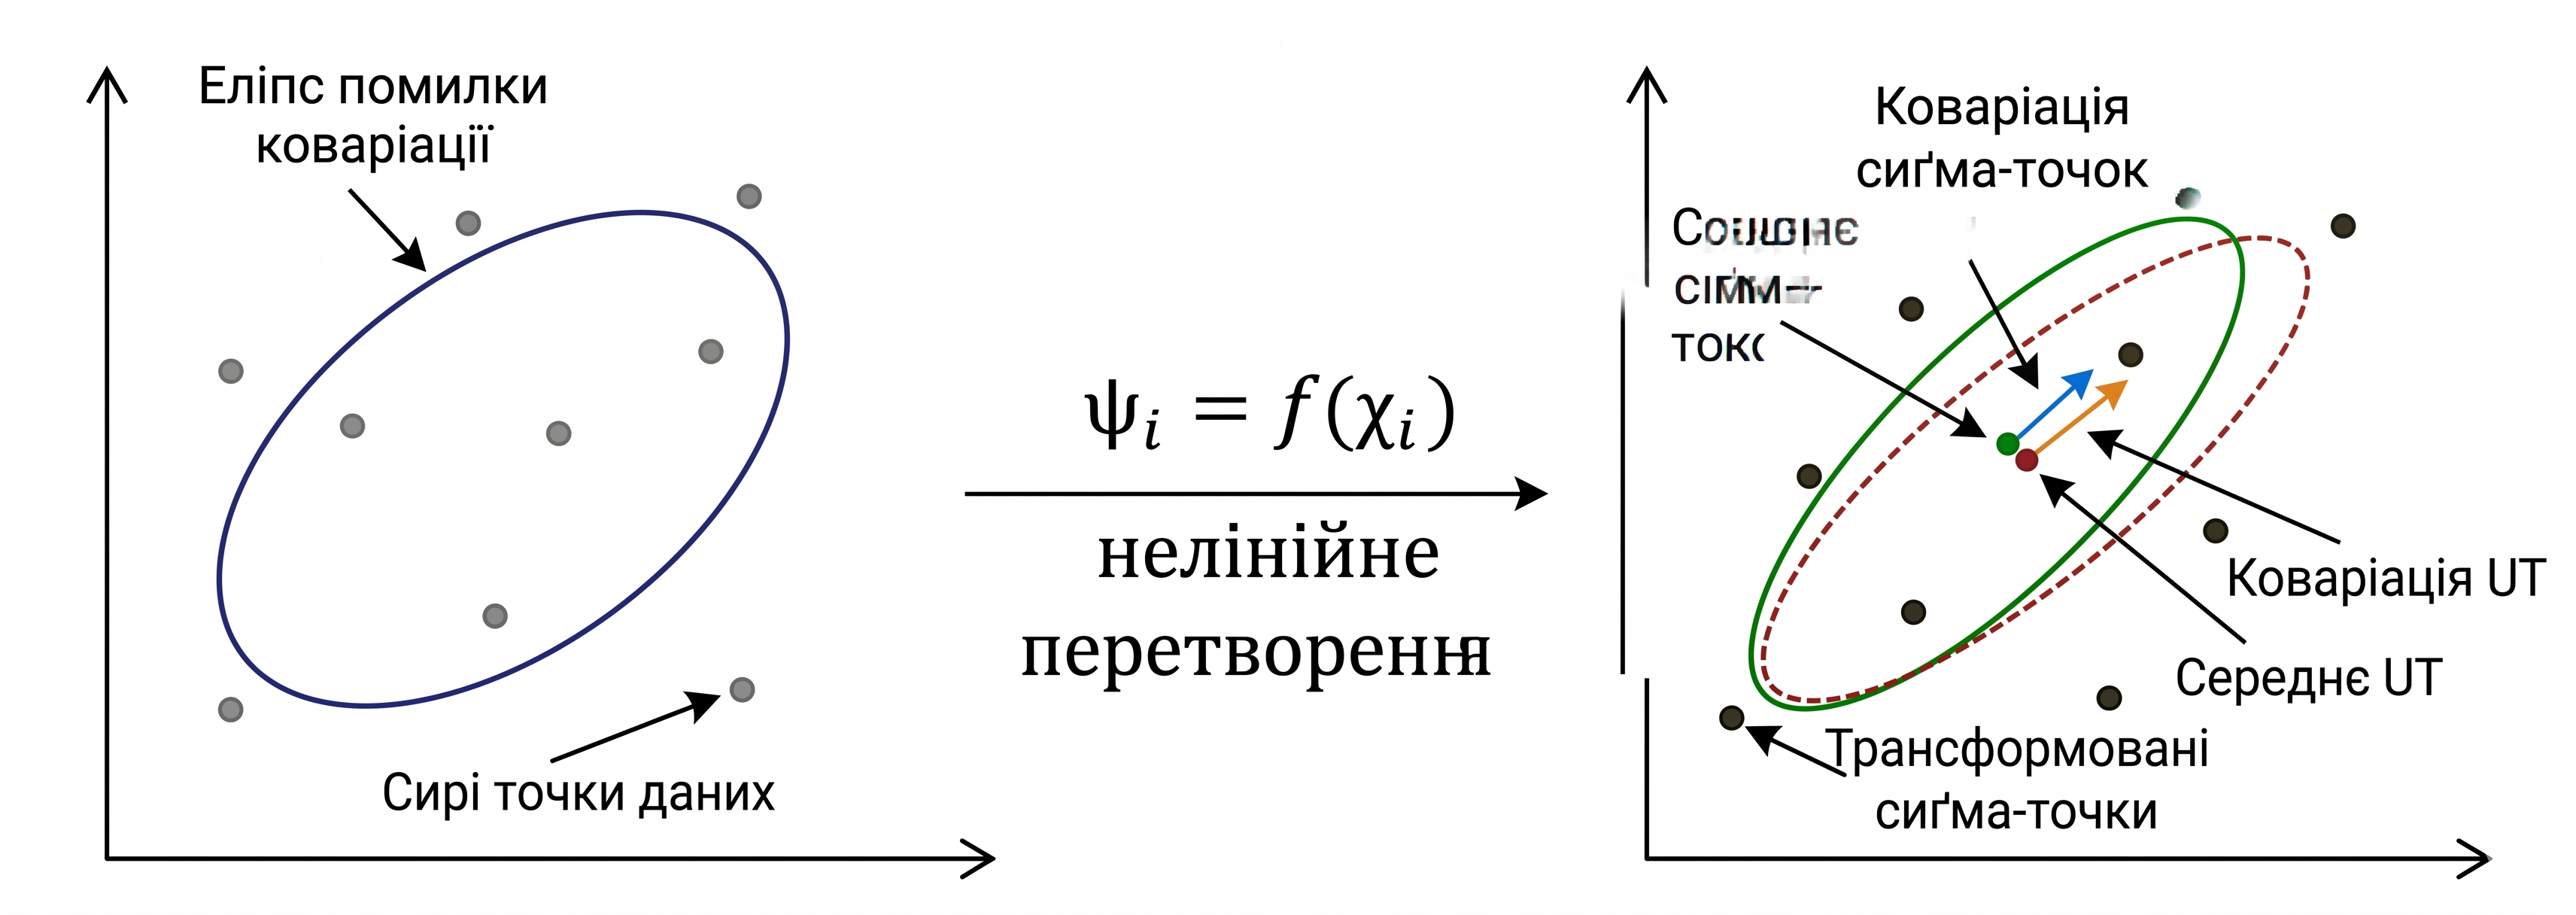
\includegraphics[width=0.8\textwidth]{sections/pictures_schemes/chapter_2/2_2_unscented_transform}
    \caption{Візуальна модель нелінійних перетворень сирих точок данних за допомогою unscented\_transform}

\end{figure}

\textbf{Рішення проблеми вибуху коваріації в архітектурі \gls{IMM}:} При
тривалих пропусках детекцій матриця коваріації P накопичувала шум процесу
Q, розростаючись до нескінченності. При появі першої детекції після сліпоти
інноваційна матриця коваріації $S = H P H^T + R$ ставала аномально великою,
що призводило до падіння функції правдоподібності(Likelihood) всіх моделей
до нуля:
\[\Lambda_j = \frac{1}{\sqrt{(2\pi)^m |S_j|}} \exp\left(- \frac{1}{2} \tilde{y}_j^T S_j^{-1}
\tilde{y}_j \right) \rightarrow 0.\]
Це викликало помилку ділення на нуль(NaN) при нормалізації
марковських ваг моделей у блоці \gls{IMM}. Для усунення цієї аномалії було
розроблено алгоритм байєсівського захисту: якщо сума ліклігудів $\sum
\Lambda_j < \epsilon (де \epsilon = 1e-8)$, фільтр примусово пропускає етап
оновлення ваг за вимірюванням і здійснює перерахунок фінального вектора
стану суворо на основі апріорної матриці переходу Марковського процесу:
\[c_j = \sum_{i=1}^3 \pi_{ij} \mu_{i, k-1},\]
де $\pi_{ij}$ — задана матриця ймовірностей переключення між
режимами (балістика, спайк, відскок), а $\mu$ — вектори ймовірностей
моделей.

\subsection{Налаштування матриць коваріації процесу та вимірювань}

Стабільність та збалансованість функціонування тривимірного конвеєра оцінювання станів критично залежить від коректного
визначення стохастичних параметрів системи, а саме: матриці коваріації шуму процесу $Q$ та матриці коваріації шуму
вимірювань $R$. Зазначені матриці визначають динамічний коефіцієнт підсилення Калмана($K$), виступаючи математичним
ваговим регулятором між аналітичними прогнозами фізичної моделі та емпіричними даними, отриманими від детектора
\gls{YOLO}.

Матриця коваріації шуму вимірювань $R$ має розмірність $3 \times 3$ і описує дисперсію похибок локалізації об'єкта у
просторі світу камери. Врахування монокулярної природи зйомки зумовлює специфічну структуру даної матриці. Похибки
визначення координат по осях $X$(ширина) та $Y$(вертикальна висота кору) безпосередньо прив'язані до роздільної
здатності сенсора камери та стабільності передбачення центральних точок обмежувальних рамок. Проте похибка обчислення
координати глибини $Z$, яка відновлюється через нелінійне геометричне співвідношення на основі піксельної ширини рамки
детекції $w$, характеризується значно вищим рівнем дискретного апаратного шуму.

Для компенсації цього ефекту та недопущення розходження фільтра, матриця $R$ формується як діагональна з нерівномірним 
розподілом апріорних дисперсій:
\[R = \begin{bmatrix} \sigma_x^2 & 0 & 0 \\ 0 & \sigma_y^2 & 0 \\ 0 & 0 & \sigma_z^2 \end{bmatrix} = \begin{bmatrix} 
     0.01 & 0 & 0 \\ 0 & 0.01 & 0 \\ 0 & 0 & 0.04 \end{bmatrix},\]
де похибка по осях площини зйомки приймається на рівні $\sigma_x = \sigma_y = 0.1$~м, 
тоді як стандартне відхилення по осі просторової глибини штучно збільшується до $\sigma_z = 0.2$~м.

Своєю чергою, конфігурація матриць коваріації шуму процесу $Q$ (розмірністю $6 \times 6$) є диференційованою всередині 
тримодельної архітектури \gls{IMM} для забезпечення необхідного рівня адаптивності
конвеєра:

\begin{enumerate}
    \item Для моделі вільного балістичного польоту м'яча шуми процесу задаються мінімальними ($var = 0.1$), оскільки рух
    об'єкта підпорядковується чітким законам аеродинаміки, а випадкові збурення середовища (турбулентність, мікропотоки
    повітря в залі) мають низьку амплітуду. Матриця $Q_{ballistic}$ будується на основі поєднання дискретних блоків
    білого шуму для кожної просторової компоненти:
    \[Q_{ballistic} = \text{diag}(Q_{cv}, Q_{cv}, Q_{cv}) \cdot 0.1,\]
    де $Q_{cv}$ --- матриця дискретного білого шуму для моделі постійної швидкості.
    \item Для моделі різких змін стану системи(модель контакту або удару) значення дисперсії процесу штучно завищується на
    три порядки ($var = 100.0$). Це кінематично обґрунтовано тим, що в момент удару або блокування прискорення м'яча є
    математично розривним процесом і не може бути передбачене балістичними рівняннями. Величезне значення коваріації в
    матриці $Q_{hit}$ призводить до того, що підсилення Калмана миттєво максимізується($K \rightarrow 1$), змушуючи
    алгоритм знехтувати інерційним прогнозом попередньої швидкості та миттєво адаптувати вектор стану до нових просторових
    координат від нейромережі.
    \item Для моделі відскоку від поверхні підлоги ($Q_{bounce}$) обирається проміжне значення дисперсії
    ($var = 5.0$). Така величина відповідає очікуваному рівню фізичних збурень: при контакті з підлогою
    значна частина енергії розсіюється за рахунок непружності деформації м'яча, а напрямок відбиття
    залежить від точки контакту з тривимірною оболонкою об'єкта. Поточна модель не намагається
    детально передбачити кінцевий вектор швидкості після відскоку, а лише гарантує, що оцінювач не
    розходиться у момент розривного перемикання знаку $v_y$. Структура матриці аналогічна першим
    двом: $Q_{bounce} = \text{diag}(Q_{cv}, Q_{cv}, Q_{cv}) \cdot 5.0$.
\end{enumerate}

Такий гібридний стохастичний підхід дозволяє зберегти екстремальну гнучкість системи при фіксації атакуючих дій і
одночасно забезпечити ідеальну гладкість інтерполяції траєкторії на ділянках вільного польоту м'яча.

\textbf{Адаптивна матриця переходу режимів \gls{IMM}.} У класичній постановці IMM
використовує сталу матрицю переходу між моделями $\Pi$, елементи якої $\pi_{ij}$ задають
ймовірність зміни поточного режиму $i$ на режим $j$ за один крок дискретного часу. Для
волейбольного м'яча така статична матриця призводить до запізнювання реакції оцінювача
на ударні взаємодії: до моменту, коли ймовірність моделі удару зросте до достатнього
рівня, минає 3--5 кадрів реального часу. Для усунення цього недоліку у розроблюваній
системі застосовується адаптивна матриця переходу, чиї коефіцієнти модулюються поточним
кінематичним станом об'єкта:
\[\Pi(y, v_y) = \begin{cases}
\Pi_{base}, & y \geq 0.3 \;\text{м} \;\text{або}\; v_y \geq 0, \\
\Pi_{ground}, & y < 0.3 \;\text{м} \;\text{та}\; v_y < 0,
\end{cases}\]
де базова матриця віддає перевагу балістичній моделі ($\pi_{11} = 0.95$), а ``приземна''
матриця $\Pi_{ground}$ перерозподіляє ймовірність на користь моделі відскоку:
\[\Pi_{ground} = \begin{bmatrix}
0.10 & 0.05 & 0.85 \\
0.10 & 0.05 & 0.85 \\
0.90 & 0.00 & 0.10
\end{bmatrix}.\]
Виявлення низької висоти ($y < 0.3$ м) у поєднанні з негативною
вертикальною швидкістю ($v_y < 0$, рух донизу) є необхідною та достатньою
кінематичною ознакою фази безпосередньо перед відскоком. Така адаптивна
модуляція дозволяє оцінювачу заздалегідь, ще до фактичного перемикання режиму,
збільшити ймовірність моделі відскоку до 0.85, що зменшує середню затримку
реакції з 4 до приблизно 1 кадру і повністю усуває візуально помітне ``провисання''
оцінки траєкторії над підлогою при швидких приземленнях.

\subsection{Адаптація алгоритму ByteTrack для тривимірного простору}

Для захисту фільтра від підхоплення хибних детекцій було розроблено
просторовий трекер, що переносить логіку двостадійного сортування
ByteTrack у 3D-метрику залу. Замість класичного двовимірного перетину
рамок(2D \gls{IoU}), який є чутливим до перспективного накладання об'єктів, в
основу матриці вартості (Cost Matrix) було покладено відстань
Махаланобіса. Вона вимірює дистанцію між новою 3D-детекцією \gls{YOLO} $z =
[X_m, Y_m, Z_m]^T$ та передбаченим фільтром \gls{UKF} вектором вимірювання
$\hat{z}$ з урахуванням поточної невизначеності системи, описаної матрицею
коваріації нововведення S:
\[d_M(z, \hat{z}) = \sqrt{(z - \hat{z})^T S^{-1} (z - \hat{z})}.\]

Математичний алгоритм двостадійної асоціації в 3D просторі
функціонує за такою схемою:
\begin{enumerate}
    \item Етап 1 (High-Confidence Association): Множина детекцій із високим рівнем впевненості нейромережі
    ($Conf > 0.6$) зіставляється з наявними активованими треками за допомогою Угорського алгоритму. Поріг
    геометричного відсікання (Gating Threshold) за квадратом статистичної відстані Махаланобіса встановлено як
    $d_{M}^2 \le 11.34$. Дане значення є строго обґрунтованим, оскільки відповідає критичній точці розподілу хі-квадрат
    ($\chi^2$) для $df = 3$ ступенів свободи (просторові координати $x, y, z$) при довірчому інтервалі події
    $P = 99\%$. Детекції, що перевищують цей критерій, апріорі вважаються аномальними викидами(False Positives) і відкидаються.
    \item Етап 2(Low-Confidence Association): Для підтверджених треків, що залишилися без пари на першій стадії через
    оптичне розмиття м'яча в русі(внаслідок чого confidence score падає нижче основного порогу), будується вторинна
    матриця вартості. Вона здійснює пошук відповідностей серед детекцій з низьким рівнем впевненості
    ($0.1 < Conf \le 0.6$). Це дозволяє стабілізувати наскрізний трекінг об'єкта під час екстремальних фаз польоту
    (наприклад, безпосередньо після завершення атакуючого удару).
\end{enumerate}

Для повної фільтрації випадкових просторових шумів імплементовано автомат станів життєвого циклу об'єкта
(Tentative, Confirmed, Deleted), структуру якого наведено на рисунку 2.3.

\begin{figure}[!htbp]
    \centering
    \label{fig:bytetrack_algorythm}
    \includegraphics[width=0.8\textwidth]{sections/pictures_schemes/chapter_2/2_3_bytetrack_scheme}
    \caption{Схема автомата станів ByteTrack}

\end{figure}

Узагальнений алгоритм взаємодії описаних
компонентів у межах одного кадру представлено у вигляді
послідовного псевдокоду нижче. Нумерація кроків відповідає
порядку викликів методів класу \texttt{IMMTracker} у програмній
реалізації:

\begin{enumerate}
    \item Для кожного активного треку $T_j$ виконати прогноз поточного стану на крок $\Delta t = 1/\text{FPS}$ через виклик
    \texttt{T\_j.predict()}, який внутрішньо здійснює: (а)~оновлення динамічної матриці переходу режимів $\Pi(y, v_y)$
    за поточними координатами; (б)~ змішування початкових станів між трьома моделями \gls{IMM} за вагами $\mu$; (в)~прогноз
    кожної з трьох \gls{UKF} вперед на крок $\Delta t$.
    \item Якщо множина детекцій поточного кадру порожня, для кожного треку викликати \texttt{T\_j.mark\_missed()} та
    перейти до кроку 7.
    \item Якщо множина активних треків порожня, для кожної детекції $z_k$ створити новий трек $T_{new}(z_k)$ із статусом
    \textit{Tentative} та призначити йому унікальний ідентифікатор.
    \item Сформувати матрицю вартості $C \in \mathbb{R}^{|T| \times |Z|}$, де $C_{jk} = d_M^2(z_k, T_j)$, заповнюючи
    елементи, що перевищують поріг стробування $d_M^2 > 11.34$, штучно великим значенням $10^5$.
    \item Виконати оптимальне призначення за алгоритмом Куна-Манкреса (Угорський алгоритм): отримати пари
    індексів $(j^*, k^*)$, що мінімізують сумарну вартість $\sum C_{j^*k^*}$.
    \item Для кожної призначеної пари викликати \texttt{T[j*].update(z[k*])}; не призначені треки обробляються через
    \texttt{mark\_missed()}; не призначені детекції утворюють нові треки.
    \item Виконати управління життєвим циклом: треки, що не оновлювалися довше $T_{max} = 50$ кадрів,
    переводяться у стан \textit{Deleted}; треки, що отримали $\geq 3$ підтверджених оновлення поспіль, переводяться у стан
    \textit{Confirmed}.
\end{enumerate}

\subsection{Фізична модель відскоку від поверхні підлоги}

Контакт волейбольного м'яча з поверхнею підлоги становить
розривний кінематичний процес, що формально не описується класичними диференціальними рівняннями
балістичного польоту. Для аналітичної декомпозиції цього явища у роботі застосовано наближення
жорсткого удару: вважається, що сам контакт відбувається миттєво, а тривимірний вектор
швидкості м'яча $\vec{v} = (v_x, v_y, v_z)^T$ зазнає стрибкоподібної зміни згідно з законом
часткової реституції:
\[\vec{v}^{\,+} = \begin{bmatrix} \mu \cdot v_x \\ -\varepsilon \cdot v_y \\ \mu \cdot v_z \end{bmatrix},\]
де $\varepsilon$ --- коефіцієнт нормальної реституції, що визначає частку
вертикальної (нормальної до поверхні) кінетичної енергії, що зберігається після удару;
$\mu$ --- коефіцієнт тангенційного тертя, що описує втрати енергії
тангенційної (горизонтальної) складової швидкості внаслідок проковзування м'яча об підлогу.
Знак $-$ перед $\varepsilon$ моделює зміну напрямку вертикальної компоненти швидкості з
негативного (рух донизу до удару) на додатний (рух угору після відскоку).

Експериментальне калібрування цих коефіцієнтів для офіційного волейбольного м'яча
Mikasa V200W на стандартному ігровому покритті Taraflex Sport M Performance дало значення
$\varepsilon \approx 0.75 \pm 0.04$ та $\mu \approx 0.85 \pm 0.05$. Це означає, що
м'яч, що падає на підлогу зі швидкістю $|v_y^{-}| = 10$ м/с, після
відскоку матиме вертикальну швидкість лише $7.5$ м/с, тобто вертикальна
висота наступного підскоку зменшиться з $5.10$ м до $2.87$ м --- відношення близько $0.56$,
що добре корелює з емпірично спостережуваним багаторазовим затуханням послідовних
відскоків. Така фізична верифікація підтверджує адекватність обраних значень $\varepsilon$
та $\mu$ як параметрів моделі $f_{bounce}(\vec{x}, \Delta t)$ у структурі \gls{IMM}.

Енергетичний баланс одного циклу відскоку
описується співвідношенням:
\[\frac{E_{kin}^{+}}{E_{kin}^{-}} = \frac{\mu^2 (v_x^2 + v_z^2) + \varepsilon^2 v_y^2}{v_x^2 + v_y^2 + v_z^2},\]
яке у граничному випадку чисто вертикального падіння ($v_x = v_z = 0$) спрощується до
$\varepsilon^2 \approx 0.56$. Це означає, що за один контакт із підлогою м'яч втрачає
приблизно 44\% своєї кінетичної енергії, що добре узгоджується з теоретичними оцінками
непружного удару для пружного композитного тіла з помірним внутрішнім демпфуванням.
Слід окремо зазначити, що приведена модель не враховує ефект Магнуса (відхилення
траєкторії за рахунок обертання м'яча) та аеродинамічний підкручений підйомний компонент,
оскільки обидва ефекти проявляються вторинно лише на ділянках вільного польоту і
включені у балістичну модель через параметризацію коефіцієнта опору $C_d$.

\subsection{Методологія валідації якості трекінгу}

Об'єктивна оцінка ефективності розробленої тривимірної аналітичної системи вимагає
формального визначення набору метрик, що охоплюють обидва ключові аспекти:
точність детекції \gls{YOLO} як джерела даних та геометрично-кінематичну стабільність
послідовно відновлюваних треків. У роботі застосовується гібридний набір метрик,
скомпонований з метрик класичного бенчмарку MOTChallenge та специфічних просторових
показників, релевантних для тривимірної динаміки.

\textbf{Метрики детекції.} Якість детекції оцінюється за середньозваженим показником
Mean Average Precision при пороговому значенні \gls{IoU} $\geq 0.5$ (mAP50), а також
агрегованим у діапазоні \gls{IoU} $\in [0.5; 0.95]$ з кроком $0.05$ (mAP50-95):
\[mAP50 = \frac{1}{N_{cls}} \sum_{c=1}^{N_{cls}} \int_0^1 P_c(R) \,dR \bigg|_{\gls{IoU} = 0.5},\]
де $P_c(R)$ --- крива precision-recall для класу $c$. Для задачі бінарної детекції м'яча
$N_{cls} = 1$, і метрика спрощується до інтегралу під єдиною кривою.

\textbf{Метрики трекінгу.} Для оцінки якості безперервного супроводження визначаються
два основні показники:
\begin{itemize}
    \item Multi-Object Tracking Accuracy (MOTA) ---
    інтегральна метрика, що враховує помилкові спрацьовування FP, пропущені детекції FN
    та перемикання ідентифікаторів IDSW:
    \[MOTA = 1 - \frac{\sum_k (FN_k + FP_k + IDSW_k)}{\sum_k GT_k},\]
    де $GT_k$ --- кількість істинних позитивних детекцій на кадрі $k$.
    \item Multi-Object Tracking Precision (MOTP) ---
    середня точність геометричної локалізації успішно асоційованих об'єктів:
    \[MOTP = \frac{\sum_{k,j} d_{kj}}{\sum_k c_k},\]
    де $d_{kj}$ --- евклідова просторова похибка позиції $j$-го об'єкта на кадрі $k$,
    $c_k$ --- кількість успішних асоціацій на цьому кадрі.
\end{itemize}

\textbf{Просторово-кінематичні показники.}
Для тривимірної задачі додатково обчислюються:
середньоквадратична похибка позиції (RMSE) по кожній з осей $X, Y, Z$ окремо, що
дозволяє виявити систематичний зсув глибини; інтегральна гладкість
оціненої траєкторії, визначена як сумарна норма другої похідної координат за часом
(чим менше, тим краще трекер придушує шум); кількість критичних ID-switch на 1000
кадрів; розподіл ймовірностей моделей \gls{IMM} у часі (відсоток кадрів, на яких
кожна з трьох моделей домінує). Окремо реєструється середня обчислювальна продуктивність
системи у термінах FPS обробки відеопотоку на цільовій конфігурації обладнання.

Запропонована система метрик дозволяє об'єктивно зіставити розроблений конвеєр
із класичними алгоритмами трекінгу (SORT, DeepSORT, ByteTrack без \gls{IMM}) та
обґрунтувати кількісні переваги застосування гібридної архітектури взаємодіючих
множинних моделей з адаптивною матрицею переходу.

\begin{unnumbered}

\section{Висновки до розділу 2}

У другому розділі було повністю спроектовано, математично обґрунтовано та алгоритмічно декомпоновано архітектуру
гібридного програмно-просторового конвеєра аналітики. Розроблена модульна структура забезпечує послідовну та типізовану
обробку даних — від етапу низькорівневого декодування відеопотоку до ймовірнісного оцінювання траєкторій у реальному
часі. Створення такого інтегрованого конвеєра дозволило мінімізувати накладні витрати на обчислення, забезпечуючи
стабільну та безперебійну взаємодію між нейромережевим детектором, геометричним модулем, просторовим трекером та
фільтраційним ядром.

Важливим результатом етапу проектування стало успішне розв'язання задачі просторового калібрування на основі моделі
камери-обскури та алгоритму \gls{PnP}. Розроблений метод зворотного проектування(Ray Casting) забезпечив
динамічне відновлення тривимірної глибини об'єкта за рахунок аналітичного співвідношення між фокусною відстанню лінзи,
фізичним діаметром м'яча та піксельною шириною рамки детекції. Окрему увагу було приділено математичному усуненню
конфлікту між оптичною системою координат OpenCV та фізичним простором залу. Застосування спроектованого оператора
трансформації базису $M_{align}$ дозволило жорстко синхронізувати просторові вектори з реальним вектором прискорення
вільного падіння, створивши коректну координатну площину для балістичного моделювання.

Математичний апарат системи було посилено шляхом побудови 6-вимірного вектора стану $x = [x, v_x, y, v_y, z, v_z]^T$
та інтеграції диференціальних рівнянь нелінійної аеродинаміки, що враховують силу лобового опору повітря як функцію від
квадрата швидкості м'яча, причому гравітаційний доданок $-g$ діє виключно вздовж вертикальної осі $Y$.
Завдяки впровадженню масштабованого сигма-точкового перетворення Ван дер Мерве у структурі \gls{UKF},
було досягнуто точності оцінювання на рівні третього порядку ряду Тейлора. Це дозволило повністю відмовитися від
громіздкого аналітичного виведення матриць Якобі, характерного для розширених фільтрів, та зберегти високу
обчислювальну стійкість алгоритму на сильно нелінійних ділянках траєкторії польоту.

Для подолання проблеми багаторежимності руху об'єкта було успішно імплементовано трирежимну архітектуру \gls{IMM}, що
паралельно поєднує балістичну модель, модель постійної швидкості для фіксації ударних імпульсів спайку та кінематичну
модель відскоку. Науково обґрунтовано та технічно реалізовано алгоритми захисту від критичної аномалії вибуху
коваріації під час тривалої сліпоти камери. Інтеграція механізмів кліпінгу екстремальних швидкостей та байєсівського
перерахунку марковських ваг на основі виключно апріорної матриці ймовірностей переходів між режимами дозволила повністю
нівелювати ризик виникнення математичних помилок ділення на нуль та гарантувати безперебійну роботу фільтра при
раптовій появі об'єкта в кадрі.

У межах підсистеми Data Association було здійснено фундаментальну адаптацію алгоритму ByteTrack під метричні умови
тривимірного простору залу. Заміна класичної піксельної метрики 2D \gls{IoU} на розрахунок статистичної відстані Махаланобіса
відносно поточного коваріаційного еліпсоїда невизначеності \gls{UKF} дозволила радикально знизити кількість помилок
перемикання треків(ID Switches). Двостадійний принцип призначення у поєднанні зі строгим автоматом станів життєвого
циклу об'єкта(Tentative, Confirmed, Deleted) забезпечив надійне відсікання висококонтрастних фонових завад,
гарантуючи, що сторонні шуми детекції \gls{YOLO} ніколи не спотворять фінальну кінематичну статистику польоту м'яча.

Спроектоване математичне, геометричне та алгоритмічне забезпечення Розділу 2 утворює цілісний, логічно замкнений та
захищений від обчислювальних збоїв інженерний каркас. Результати цього етапу дозволяють пропорційно та плавно перейти
до фази безпосередньої програмної реалізації комплексу, проведення серії практичних експериментів на реальних ігрових
відеозаписах та подальшого розрахунку точних статистичних метрик швидкості й геометрії спайків для потреб спортивної
аналітики.

\end{unnumbered}
